\clearpage
\phantomsection
%\addcontentsline{toc}{chapter}{مقدمات}
\chapter{پیاده سازی و نتایج}
\markboth{پیاده سازی و نتایج}{عنوان فصل}

در این بخش ابتدا پیاده‌سازی مدل نورونی را انجام داده سپس اول از نورون ساخته‌شده در یک شبکه عصبی پیشرو استفاده می‌کنیم و در مرحله بعد معماری شبکه عصبی اسپایکی پیچشی را با مدل نورونی نشت کننده و ادغام آتش پیاده سازی کرده و در نهایت الگوریتم خودنظارتی را به ساختار شبکه اضافه می‌کنیم و نتایج را برای داده های MNIST و CIFAR10 مشاهده و بررسی خواهیم کرد.


\section{پیاده سازی مدل نورونی}

 در ابتدا مدل نورونی را با توجه به آنچه در فصل یک توضیح داده شد پیاده‌سازی کرده و تغییرات پتانسیل و فرآیند تولید اسپایک را بررسی می‌کنیم. همانطور که گفته شد بعد خروجی مدل نورونی برابر است با  :
 
\[
\left[ \text{time step} \times \text{batch size} \times \text{feature dimension} \right]
\]

  و با توجه به اینکه بعد زمان در تانسور خروجی وجود دارد و داده به عنوان جریان ثابت به شبکه در طول گام های زمانی داده شده است, برای بررسی روند تولید اسپایک, تغییرات پتانسیل هر نورون را در طول گام‌های زمانی جمع بسته و بررسی می‌کنیم آیا پتانسیل از آستانه عبور کرده یا خیر.
در شکل  \ref{fig:liff} یک نمونه از جریان ثابت ورودی و یک نمونه از خروجی نورون که شامل تغییرات پتانسیل و گسیل اسپایک می‌شود نشان داده‌شده است.

\begin{minipage}{\linewidth}
	\centering
	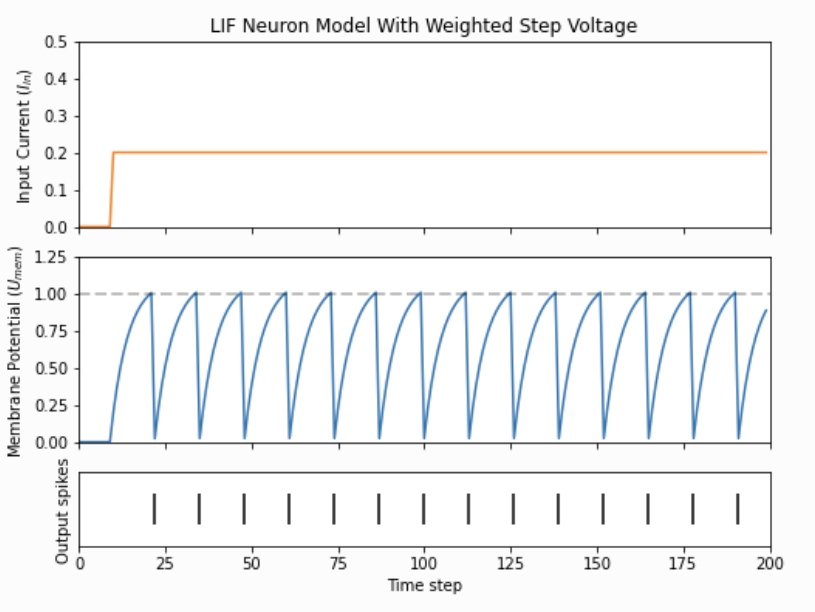
\includegraphics[width=8cm]{lif.png}
	\captionsetup{font=small} % Adjust the font size of the caption
	\captionof{figure}{پیاده‌سازی مدل نورونی نشت‌کننده و ادغام آتش ونمایش تولید اسپایک در صورت عبور پتانسیل از آستانه}
	\label{fig:liff}
\end{minipage}







\section{پیاده سازی یادگیری خودنظارتی روی شبکه عصبی اسپایکی}
برای ساخت اتصالات بین نورون ها از اتصالات پیچشی و کاملا متصل استفاده می‌کنیم به این صورت که لایه‌های اسپایکی خروجی‌های اسپایک و تغییرات پتانسیل غشا را تولید می‌کنند و لایه‌های پیچشی و کاملا متصل نوع اتصال نورون ها را مشخص می‌کنند.
% ساختار شبکه به صورت زیر است :
%
%1. لایه پیچشی ۱ (conv1):
%
%این لایه یک لایه پیچشی دوبعدی است که ورودی‌های ۳ کانال را به ۳۲ کانال تبدیل می‌کند. این لایه ورودی‌ها را با یک فیلتر به اندازه ۲در۲ کوچکتر می‌کند.
%
%2. لایه اسپایکی ۱ (lif1):
%این لایه یک لایه فعال‌سازی است که برای نورون‌های اسپایکی از آن استفاده می‌شود و بردار اسپایک و تغییرات پتانسیل را به عنوان خروجی می‌دهد.
%
%3. لایه پیچشی ۲ (conv2):
%این لایه نتایج خروجی از لایه اسپایکی قبلی را با یک فیلتر دیگر به اندازه ۲در۲ کوچکتر می‌کند و به ۶۴  کانال تبدیل می‌کند.
%
%4. لایه اسپایکی ۲ (lif2):
% این لایه نیز برای فعال‌سازی نورون‌های اسپایکی استفاده می‌شود و با پارامتر بتا تنظیم می‌شود.
%
%5. لایه پیچشی ۳ (conv3):
%این لایه به عنوان یک لایه پیچشی جدید اضافه شده است که ورودی‌ها را با یک فیلتر دیگر به ۱۲۸ کانال تبدیل می‌کند.
%
%6. لایه اسپایکی ۳ (lif3):
%همانند لایه‌های  قبلی، این لایه نیز برای فعال‌سازی نورون‌های اسپایکی اضافه شده و با تنظیم پارامتر بتا کار می‌کند.
%
%7. لایه پیچشی ۴ (conv4):
%این لایه نتایج خروجی از لایه پیچشی جدید قبلی را با یک فیلتر دیگر به اندازه ۲در۲ کوچکتر می‌کند و به ۲۵۶  کانال تبدیل می‌کند.
%
%8. لایه اسپایکی ۴ (lif4):
%همانند لایه‌های اسپایکی  قبلی، این لایه نیز برای فعال‌سازی نورون‌های اسپایکی اضافه شده است.
%
%9. لایه خطی ۱ (fc1):
%این لایه اتصالات خطی دارد و ورودی‌ها را به یک بردار ۵۱۲ بعدی تبدیل می‌کند. 
%
%10. لایه اسپایکی ۵ (lif5):
% این لایه نیز برای فعال‌سازی نورون‌های اسپایکی اضافه شده است.
%
%11. لایه خطی ۲ (fc2):
%این لایه خطی یک لایه جدید با ورودی‌های ۵۱۲ بعدی را به یک بردار ۳۲ بعدی تبدیل می‌کند.
%
%12. لایه اسپایکی ۶ (lif6):
%این لایه نیز برای فعال‌سازی نورون‌های اسپایکی اضافه شده و با تنظیم پارامتر بتا کار می‌کند. این لایه به لایه خطی ۲ اعمال می‌شود.

برای پیاده سازی بخش خودنظارتی هر بار دو نمونه از داده افزوده‌شده را در دسته‌های با اندازه‌های مختلف به شبکه داده و تابع هزینه را روی خروجی شبکه که در طول زمان جمع بسته شده اعمال می‌کنیم و فرآیند آموزش را طی می‌کنیم تا شبکه بیاموزد نمایش‌های مناسب از داده را تولید کند. نمودار تغییر تابع هزینه را در طول زمان مشاهده می‌کنیم و به این معناست که شبکه در حال آموختن است. با توجه به اینکه در این مرحله فرایند آموزش با داده بدون برچسب اتفاق می‌افتد تنها تغییر تابع هزینه بر روی مجموعه داده آموزشی  در شکل‌های  \ref{fig:loss1} و  \ref{fig:loss2}  قابل مشاهده است.


% \begin{minipage}{\linewidth}
% 	\raggedleft
% 	\includegraphics[width=8cm]{mnistloss.png}
% 	\captionof{figure}{نمودار تابع هزینه شبکه برای مجموعه داده  mnist}
% 	\label{fig:kknnn}
% \end{minipage}
% 
 
\begin{minipage}{0.49\linewidth}
	\centering
	\includegraphics[width=\linewidth]{mnistloss.png}
	\captionsetup{font=small} % Adjust the font size of the caption
	\captionof{figure}{نمودار تابع هزینه شبکه برای مجموعه داده  mnistدر فرایند یادگیری خودنظارتی}
	\label{fig:loss1}
\end{minipage}
%\hspace{0.01\textwidth}
\begin{minipage}{0.49\linewidth}
	\centering
	\includegraphics[width=\linewidth]{cifarloss.png}
	\captionsetup{font=small} % Adjust the font size of the caption
	\captionof{figure}{نمودار تابع هزینه شبکه برای مجموعه داده  cifar فرایند یادگیری خودنظارتی}
	\label{fig:loss2}

\end{minipage}




سپس برای آزمایش نمایش‌های تولید شده و آزمودن عملکرد شبکه یک بار نمایش‌ها را به عنوان ورودی به الگوریتم نزدیک‌ترین همسایه می‌دهیم و بررسی می‌کنیم و یک بار نیز  دسته‌بند را به عنوان لایه آخر به شبکه اضافه می‌کنیم و بعد نمایش خروجی را به اندازه تعداد دسته داده که در این پروژه برای هر دو مجموعه داده MNIST , CIFAR10 تعداد ۱۰ است کاهش می‌دهیم و طی یک فرایند آموزش نظارت شده دقت شبکه را می‌سنجیم.


\section{پیاده سازی الگوریتم نزدیک ترین همسایه }
از کتابخانه sklearn برای پیاده کردن الگوریتم استفاده کرده و بر روی دو مجموعه داده آزمایش کرده ایم به این صورت که چند نمایش خروجی از شبکه را به صورت تصادفی انتخاب کرده و ده همسایه نزدیک به آن را مشاهده کرده ایم . با توجه به شکل  \ref{fig:kknnn} مشاهده می‌شود که الگوریتم نزدیک ترین همسایه نمایش‌های مشابه را برای نمونه‌های تصادفی از خروجی شبکه به درستی تشخیص داده است.


\begin{minipage}{\linewidth}
	\centering
	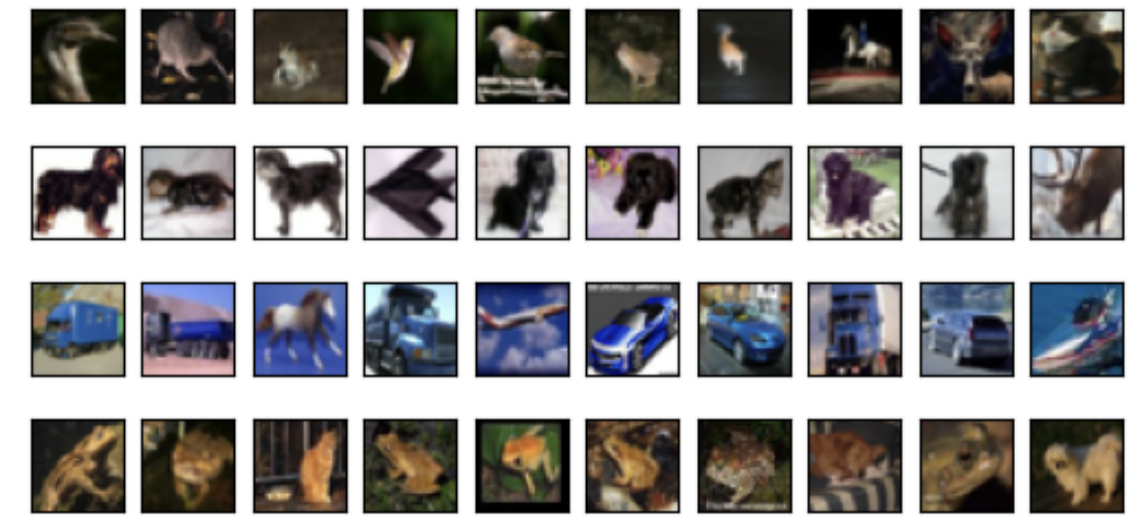
\includegraphics[width=8cm]{knnn.png}
	\captionsetup{font=small} % Adjust the font size of the caption
	\captionof{figure}{نمونه خروجی الگوریتم نزدیک ترین همسایه بر روی نمایش های تولید شده توسط شبکه عصبی اسپایکی در طول یادگیری خودنظارتی}
	\label{fig:kknnn}
\end{minipage}



\section{  پیاده سازی دسته بندی کننده و نتایج }

برای اضافه کردن دسته‌بندی‌کننده از یک لایه خطی کاملا متصل استفاده می‌کنیم که بعد تانسور خروجی را به تعداد دسته‌ها در داده کاهش می‌دهد و با جمع بستن خروجی در طول زمان هر درایه‌ای در تانسور خروجی اسپایک که بیشترین فعالیت را داشته باشد به عنوان برچسب مربوط به آن داده در نظر گرفته می‌شود. لازم به ذکر است چون یکی از اهداف مهم یادگیری خودنظارتی کم کردن نیاز به داده برچسب دار است در این مرحله از فرآیند آموزش شبکه با حدود ۲۰٪ از حجم داده اصلی آموزش می‌بیند. در صورتی که ۸۰٪ از داده برای آموزش خودنظارتی شبکه استفاده شده است.
در شکل‌های \ref{fig:closs1} و  \ref{fig:closs2}  تغییر تابع هزینه در طول فرآیند یادگیری نظارت شده را مشاهده می‌کنیم.


\begin{minipage}{0.49\linewidth}
	\centering
	\includegraphics[width=\linewidth]{cmnist.png}
	\captionsetup{font=small} % Adjust the font size of the caption
	\captionof{figure}{نمودار تابع هزینه شبکه برای مجموعه داده  MNIST فرایند یادگیری نظارت شده با ۲۰٪ حجم داده}
	\label{fig:closs1}
\end{minipage}
%\hspace{0.01\textwidth}
\begin{minipage}{0.49\linewidth}
	\centering
	\includegraphics[width=\linewidth]{ccifar.png}
	\captionsetup{font=small} % Adjust the font size of the caption
	\captionof{figure}{نمودار تابع هزینه شبکه برای مجموعه داده  CIFAR فرایند یادگیری نظارت شده با ۲۰٪ حجم داده}
	\label{fig:closs2}
	
\end{minipage}

پارامترهایی همچون اندازه دسته , انتخاب روش افزودن داده و تعداد گام زمانی در عملکرد نهایی شبکه تاثیرگذارند. در جدول‌های زیر آزمایش‌های انجام شده برای مشاهده تاثیر هر یک از پارامتر‌ها نشان داده شده است. 





\begin{table}[h!]
	%\caption{Multi-column Table}
	\centering
	\begin{tabular}{|c |c c| rrrrrrr}
			\hline
		اندازه دسته & MNIST & CIFAR10    \\ 
		\hline
		64   & 45.77    &76.52     \\
		%\hline
		128    & 87.79     & 28.55      \\
		%\hline
		256   & 13.82     & 79.58         \\
		\hline
		
	\end{tabular}
	\captionsetup{font=small} % Adjust the font size of the caption
	\caption{ درصد دقت عملکرد شبکه با توجه به اندازه دسته‌های مختلف}
\end{table}



\begin{table}[h!]
	%\caption{Multi-column Table}
	\centering
	\begin{tabular}{|c |c c| rrrrrrr}
		\hline
		گام زمانی & MNIST & CIFAR10    \\ 
		\hline
		10   & 21.78     &63.53    \\
		%\hline
		20    & 54.81     & 84.57     \\
		%\hline
		30   & 34.82    & 15.58         \\
		\hline
		
	\end{tabular}
	\captionsetup{font=small} % Adjust the font size of the caption
	\caption{درصد دقت عملکرد شبکه با توجه به گام های زمانی مختلف}
\end{table}


\begin{table}[h!]
	%\caption{Multi-column Table}
	\centering
	\begin{tabular}{|c |c c| rrrrrrr}
		\hline
		روش افزودن داده & CIFAR10& MNIST     \\ 
		\hline
		برش - چرخش   & 21.55      &43.81     \\
		%\hline
		برش - نویز گاوسی    & 12.56     & 06.82      \\
		%\hline
		چرخش - نویز گاوسی   & 54.58     & 23.82          \\
		\hline
		
	\end{tabular}
	\captionsetup{font=small} % Adjust the font size of the caption
	\caption{درصد دقت عملکرد شبکه با توجه به روش‌های مختلف افزودن داده}
\end{table}






از طرفی با توجه به اینکه هدف اصلی اعمال یادگیری خودنظارتی بر روی شبکه, بی‌نیاز کردن یادگیری از داده برچسب‌دار است انتظار می‌رود پس از اعمال این فرآیند, شبکه از فرآیند یادگیری نظارت شده روی داده برچسب دار با حجم کم دقت بهتری داشته باشد.در نتیجه یک بار نیز شبکه با همان معماری را به صورت نظارت‌شده بر روی داده با حجم کم(۲۰٪ از حجم کل داده) آموزش می‌دهیم و نتایج را مقایسه می‌کنیم . 
پس از آزمایش‌های انجام شده نتیجه گرفتیم که شبکه عصبی اسپایکی با فرآیند یادگیری خودنظارتی عملکرد بهتری از آموزش نظارت شده برای داده‌های برچسب‌دار با حجم کم دارد.

در نمودارهای  \ref{fig:acc1} و  \ref{fig:acc2}دقت هریک از روش‌های خودنظارتی و نظارت شده بر روی مجموعه داده‌های MNIST , CIFAR10 نشان داده شده است.


\begin{minipage}{0.49\linewidth}
	\centering
	\includegraphics[width=\linewidth]{macc.png}
	\captionsetup{font=small} % Adjust the font size of the caption
	\captionof{figure}{مقایسه دقت عملکرد روش‌های یادگیری خودنظارتی و نظارت‌شده بر روی مجموعه داده MNIST}
	\label{fig:acc1}
\end{minipage}
%\hspace{0.01\textwidth}
\begin{minipage}{0.49\linewidth}
	\centering
	\includegraphics[width=\linewidth]{cacc.png}
	\captionsetup{font=small} % Adjust the font size of the caption
	\captionof{figure}{مقایسه دقت عملکرد روش‌های یادگیری خودنظارتی و نظارت شده بر روی مجموعه داده CIFAR10}
	\label{fig:acc2}
\end{minipage}

همانطور که مشاهده می‌شود پیاده سازی روش یادگیری خودنظارتی موجب افزایش دقت عملکرد شبکه شده‌است. و همچنان نیاز به داده برچسب‌دار را بسیار کاهش داده و با توجه به اینکه روش یادگیری خودنظارتی بر روی شبکه‌های اسپایکی اعمال شده به علت ساختار این شبکه‌ها, نیاز به مصرف انرژی برای یادگیری نیز کاهش پیدا کرده و فرایند آموزش بهینه ‌تر انجام شده است.




\section{چشم انداز پژوهشی}

 با توجه به اینکه پیاده‌سازی روش‌های یادگیری خودنظارتی بر روی شبکه‌های عصبی اسپایکی یک حوزه پژوهشی نوآورانه و جذاب محسوب می‌شود، امکانات بی‌نظیری را برای بهبود کاربردها و پیشرفت در علم و فناوری فراهم می‌کند. این پیشرفت در ارتقاء روش‌های یادگیری و استفاده از داده‌های پیچیده‌تر، می‌تواند اثرات مثبتی بر تحقیقات مختلف داشته باشد.
 با توجه به چالش کمبود داده برچسب‌دار و هزینه و زمان‌بر بودن فرآیند تولید برچسب برای داده, این چالش ممکن است مانع از استفاده کامل از روش‌های یادگیری تقویتی و عمقی شود. 
 
 از طرفی با توجه به ماهیت بیولوژیکی شبکه‌های عصبی اسپایکی و بهینه بودن آن‌ها در مصرف انرژی زمان نسبت به شبکه‌های عصبی مصنوعی, استفاده از این شبکه‌ها منجر به پیشرفت‌هایی در حوزه‌های مختلف یادگیری و علوم اعصاب خواهد شد.
 با پیاده‌سازی روش‌ یادگیری خودنظارتی بر روی شبکه‌های عصبی اسپایکی، می‌توان به صورت تخمینی و بدون نیاز به داده‌های برچسب‌دار، توانایی‌های شبکه‌ها در تشخیص الگوها و اطلاعات مهم را بهره‌برداری کرد. این روش، باعث تولید ابزاری مؤثر در ایجاد نمایندگان با کیفیت از داده‌ها می‌شود که می‌تواند در کاربردهای متعددی در زمینه‌های مختلف مانند تشخیص بیماری‌ها، پیش‌بینی تغییرات و... مفید واقع شود.
 امید است این ابزار محاسباتی در حوزه‌های مختلف یادگیری مفید واقع شود و بتوان به این وسیله در مسائل مختلف یادگیری ماشین و پردازش داده تصویری موجب پیشرفت شد.
 
 در ادامه روند این پژوهش بنا داریم با پیچیده‌تر کردن شبکه و بررسی پارامتر‌ها عملکرد شبکه را بهبود بخشیم و با افزایش دقت شبکه یک ابزار قوی و قابل اعتماد محاسباتی تولید کنیم که نه تنها نیاز به داده‌برچسب‌دار را کاهش دهد بلکه در مصرف انرژی و حافظه نیز بهینه باشد.
 